

\chapter{Mixing Python and Fortran} 
Python is considered as one of the best glues to link different languages. 
Usually, the process is to interface languages to a common complied language C
Depending on the application, two different alternatives are possible. 

Python is often described as a “glue language,” 
meaning it can let disparate code 
(typically libraries with C language interfaces) interoperate. 
Its use in data science and machine learning is in this vein,
but that’s just one incarnation of the general idea. 
If you have applications or program domains that you would like to hitch up, 
but cannot talk to each other directly, you can use Python to connect them.


\begin{enumerate}
    \item \textbf{Calling Fortran from Python}: The Fortran library is compiled and transformed to a Python module. The Python interface has 
    a complete 
    control over the Fortran module. This method allows to keep the original performance of the Fortran programme.
    
    \item \textbf{Calling Python from Fortran}: 
    The Fortran programme has a complete control and the Python library is called only when needed. Variables 
    are shared through a global dictionary instead of through the function's arguments. The performance is reduced proportionally to the 
    number of calls to the Python library.
\end{enumerate}

Each one of these approaches has its advantages and disadvantages and the use of one or other approach strongly depends on the particular 
situation and the flexibility of both solvers.

\section{Calling Fortran from Python} 
This is the most common approach. 
usually the desired approach, 
because the Python programme acts as main and it facilitates the post-processing tasks. 
Furthermore, it would allow to have control over both solvers from the same main programme, 
which simplifies the coupling process.

The key behind this methodology is to compile the Fortran programme, 
while creating intermediate interfaces which allow to call each function 
and subroutine of the Fortran module as if it was a Python function. 
In order to transform the compiled Fortran module and to create the 
intermediate interfaces, the library F2PY \cite{f2py} is used.

Although this library allows to transform Fortran programmes to Python functions, 
the Fortran code has to be written in a very specific way 
in order to make it work properly and, hence, 
it is not useful in practice. 
Therefore, we developed a \emph{Fortran parser} in a previous 
work in order to overcome this problem. The parser, called \emph{fparser} \cite{fparser}, 
is a Python-based open-source library with a simple 
and intuitive GUI which automatically rewrites the content of any Fortran module 
in order to make it compatible with F2PY. 
This way, the 
previous problem is not a constraint any more and the Fortran module can be called from Python easily. However, the resulting transformed 
Fortran module, after F2PY has been used, is difficult to be used and some experience is required in this field to extract the full potential 
of this approach. Therefore, the fparser's GUI also creates a simpler Python interface which links the main Python programme with Fortran, so 
the user only has to interact with usual Python functions. This methodology is shown schematically in Figure \ref{fig:fparser}.

The main advantage of this approach is the \emph{performance} of the transformed Fortran module. Several tests have demonstrated that the 
computational efficiency of the Fortran programme is not reduced when transformed to Python functions. This fact is specially interesting for 
those applications which require a large computational time (e.g. CFD).

However, the conjunction between F2PY and fparser has some limitations that may be an impediment for some applications:
\begin{enumerate}
    \item The Fortran programme must be formed by hierarchical modules, which may contain functions and subroutines.
    \item Object-oriented programming can be used only in low-level modules, which can not be accessible from Python.
    \item Fortran procedures can be used to use a Python function as an input to a Fortran function. However, concatenated procedures are not 
    implemented in fparser.
    \item When compiling the Fortran programme, most of the flags can not be selected by the user due to they have to be automatically tuned 
    to assure a correct compatibility with F2PY.
\end{enumerate}



\vfill 

\begin{figure}[H]
  \centering
  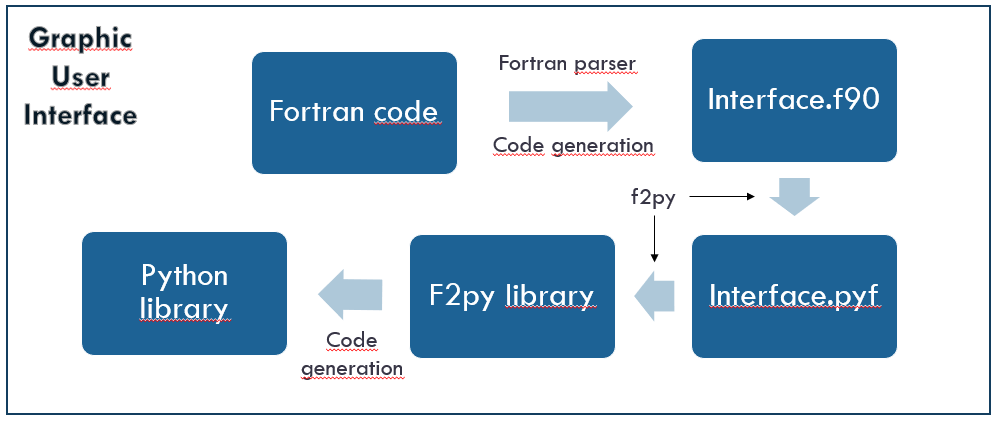
\includegraphics[width=\textwidth]{./doc/Figures/fparser.PNG}
  \caption{\normalfont{Schematics of the proposed methodology: F2PY-fparser.}}
  \label{fig:fparser}
\end{figure}

\newpage

\section{Calling Python form Fortran}

\noindent 
As an alternative to the previous approach, 
there is another way of linking a Fortran and a Python programme. 
In this case, the 
Fortran programme acts as main and, therefore, it will call the Python library when needed. The only way to do this is using \emph{compiled 
Python code}. Although Python is not designed to be compiled, there are some libraries which allow to use this functionality. In this case 
CFFI \cite{cffi} will be used to compile Python in a C-style way.

Once every Python function has been compiled, it is necessary to create some Fortran interfaces, using the \emph{iso\_c\_binding} 
functionality (included within Fortran 2003 compilers), to communicate with the C-Python code. These interfaces will be added to the Makefile 
and they will be linked to the main Fortran code during the compilation.

The main problem of this approach is that it is necessary to create a new Fortran interface with \emph{iso\_c\_binding} each time a new 
Python function is defined. This would make arduous the task of creating new Python functionalities and the setup of the coupling process 
would require a large amount of time. Therefore, it is important to avoid the creation of too many interfaces, but keeping the same 
functionality.

The equilibrium between effort and number of interfaces has been achieved by Noah Brenowitz \cite{call_py_fort}, who provides a Github 
repository with only the essential Fortran interfaces. These interfaces allow to call three predefined Python functions:
\begin{enumerate}
    \item \textbf{Set state}: Updates the value of a shared variable between Fortran and Python.
    \item \textbf{Get state}: Recovers the value of a shared variable between Fortran and Python.
    \item \textbf{Call function}: Calls an arbitrary Python function from Fortran. It only works if the Python function is installed as a 
    library within a Python environment.
\end{enumerate}

The key behind this idea is a global Python dictionary called \emph{state}, which has been defined at the interfaces to be accessible from 
Fortran and Python simultaneously. The command \emph{set\_state} updates a variable of this dictionary and \emph{get\_state} recovers the 
value of a variable. These variables are always arrays up to three-order tensors.

The command \emph{call\_function} allows Fortran to gain access to installed Python libraries. However, no input arguments can be sent 
through this command. Therefore, every Python function which needs to be called from Fortran must have a single input argument: the global 
dictionary \emph{state}. This way, the input variables can be updated from Fortran and then, when the Python function is called, it has 
access to all the predefined shared variables.

This three functions available in Fortran are enough to share any variable and to call any Python function. The scheme of this procedure is 
represented graphically in Figure \ref{fig:python_interface}.

Although this approach is restrictive from the point of view of the Python functions, it gives a complete freedom to the Fortran programme 
and no requirements are established over this language.
In the case of the solver HORSES3D, it is essential to have a lot of flexibility in the Fortran side, while the Python side can be defined as 
desired. Therefore, in this case, this is the best possible approach and it is the one that has been used in the whole research.

However, it is important to mention that the use of this approach deteriorates the computational performance of the programme. Therefore, the 
Python library has to be designed to be called a few times only, because each additional call is expensive due to the user defined Python 
functions are not compiled. However, the flexibility provided by this methodology makes it a good trade-off, even though the required time to 
run the simulations will increase.

\vfill

\begin{figure}[H]
  \centering
  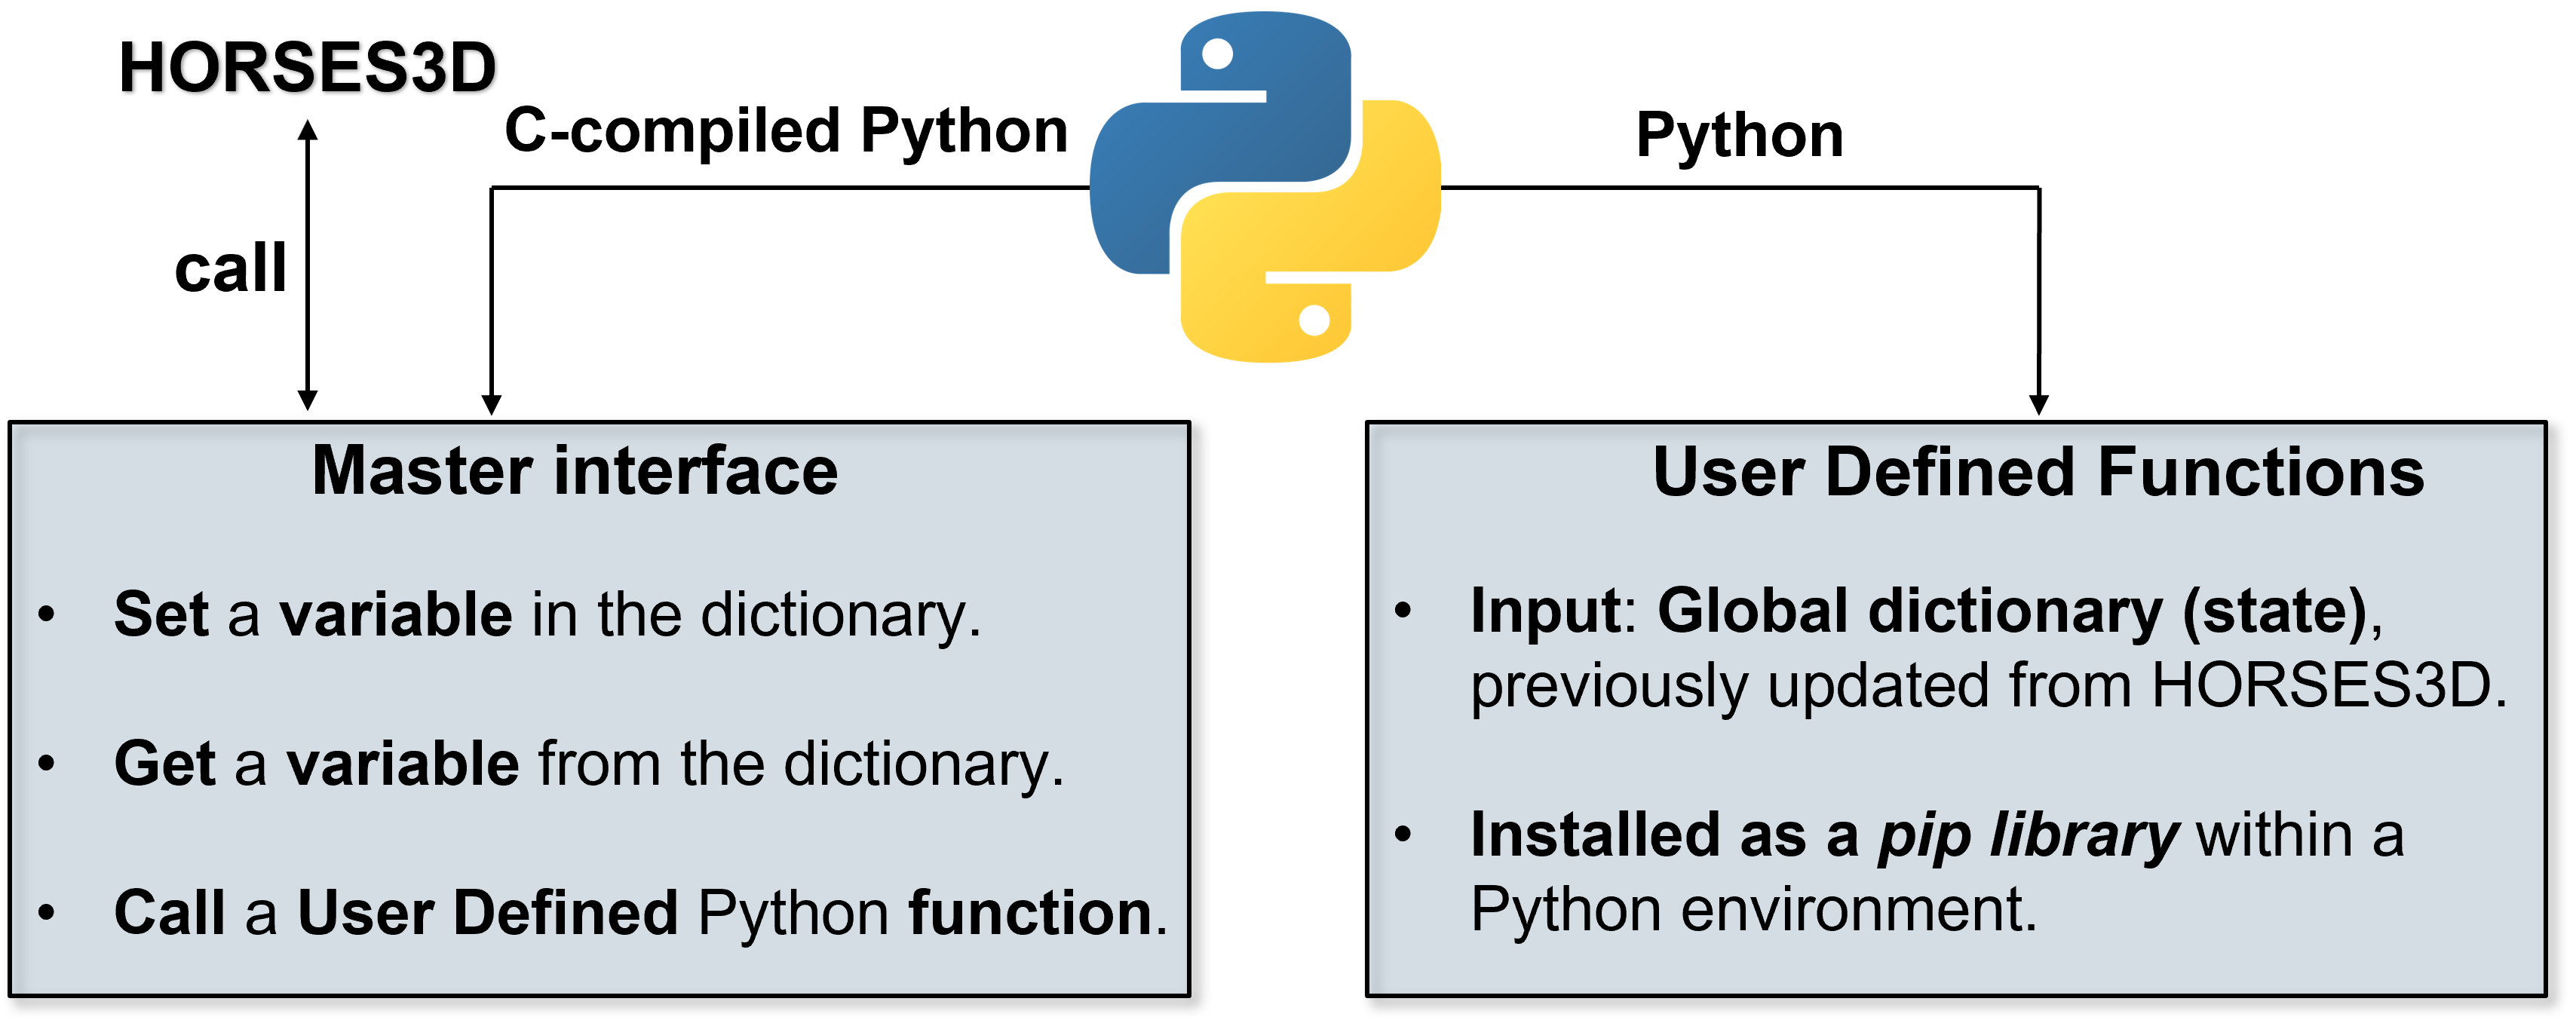
\includegraphics[width=\textwidth]{./doc/Figures/Python_interface.png}
  \caption{\normalfont{Schematics of the proposed methodology: Python interface with HORSES3D as main.}}
  \label{fig:python_interface}
\end{figure}

\vfill
